
\chapter{El transistor bipolar de unión}


\section{Introducción}


\section{Transistor bipolar ideal}

\subsection{Corrientes}

\subsection{Regiones de operacion}

\subsection{Recombinación}

\subsection{Caracterísitcas ideales IV en la zona activa}

\subsection{Ecuaciones de Ebers-Moll}


\section{Desviaciones respecto al transistor ideal}


\newpage 

% ----------------------------
% Ejercicios 
% ----------------------------

\section{Ejercicios}


%---------------------------
% Ejercicio 1
%---------------------------

\begin{Enunciado}
\subsection*{Ejercicio 1} 
Para un transistor P\textsuperscript{+}NP de silicio representar aproximadamente:
\begin{enumerate}[label=\alph*)]
    \item Bajo equilibrio las bandas, el campo eléctrico, la densidad de carga y el potencial.
    \item Las bandas en los casos de activa, corte, saturación y activa inversa.
    \item Los portadores en los casos de activa, corte, saturación y activa inversa.
\end{enumerate}
\end{Enunciado}

\vspace*{1em}

\lipsum[1].

\vspace*{2em}


%---------------------------
% Ejercicio 2
%---------------------------

\begin{Enunciado}
\subsection*{Ejercicio 2} 
Para un transistor de GaAs tipo PNP, con concentraciones $1.0 \times 10^{16}$, $5.0 \times 10^{15}$ y $1.0 \times 10^{15}$ cm\textsuperscript{-3}, con un ancho de emisor, base y colector de 20, 2 y 50 micras respectivamente, usando la aproximación de vaciamiento en los siguientes casos:
    \begin{enumerate}[label=\alph*)]
        \item Representar las bandas y el campo eléctrico en equilibrio.
        \item Representar las bandas y el campo eléctrico cuando se polariza $V_{EB} = 0.8$ V y $V_{CB} = -1.5$ V.
    \end{enumerate}
\textbf{Datos:} concentración intrínseca $2.25 \times 10^6$ cm\textsuperscript{-3}, gap de energía 1.42 eV, masa del electrón 0.066 y de hueco 0.52, permitividad relativa: 12.9, permitividad absoluta del vacío: $8.85 \times 10^{-14}$ F/cm.
\end{Enunciado}

\vspace*{1em}

Solucion: 

\begin{enumerate}[label=\alph*)]
    \item Primero vamos a presentar los valores de lal gráfico de bandas y el campo eléctrico en el equilibrio. Para esto tenemos que usar las típicas ecuaiones que hemos usado en todos los temas anteriores, y que por tanto no vamos a reptir (véase \ref{Sec:03-02}). Ahora si, tenemos algunos resultados que si tenemos que representar, que son $x_n',x_p',x_n'',x_p'',\Vbi',\Vbi''$. Recordanos que $x_n$ y $x_p$ caen con $N_D,N_A$.  Nosotros llamamos \textit{prima} a cualquier parámetro de emisor-base (EB) y \textit{doble prima} a cualquier parámetro de base-colector (BC). Así pues:
    \begin{equation}
        \text{EB:} \ x_n'=51.94 \ \mu \unit{m} \quad  x_p'=25.97  \mu \unit{m} \quad \Vbi'=1.13 \ \unit{V}
    \end{equation}
    \begin{equation}
        \text{BC:} \ x_n''=28.09 \ \mu \unit{m} \quad  x_p''=122.64  \mu \unit{m} \quad \Vbi'= 1.071 \ \unit{V}
    \end{equation}
    Y el campo eléctrico máximo
    \begin{equation}
       \abs{\Ecal'}_{\max}''=28200 \ \unit{V/cm} \quad  
       \abs{\Ecal''}_{\max}''=14100 \ \unit{V/cm} 
    \end{equation}

    \begin{figure}[h!] \centering
        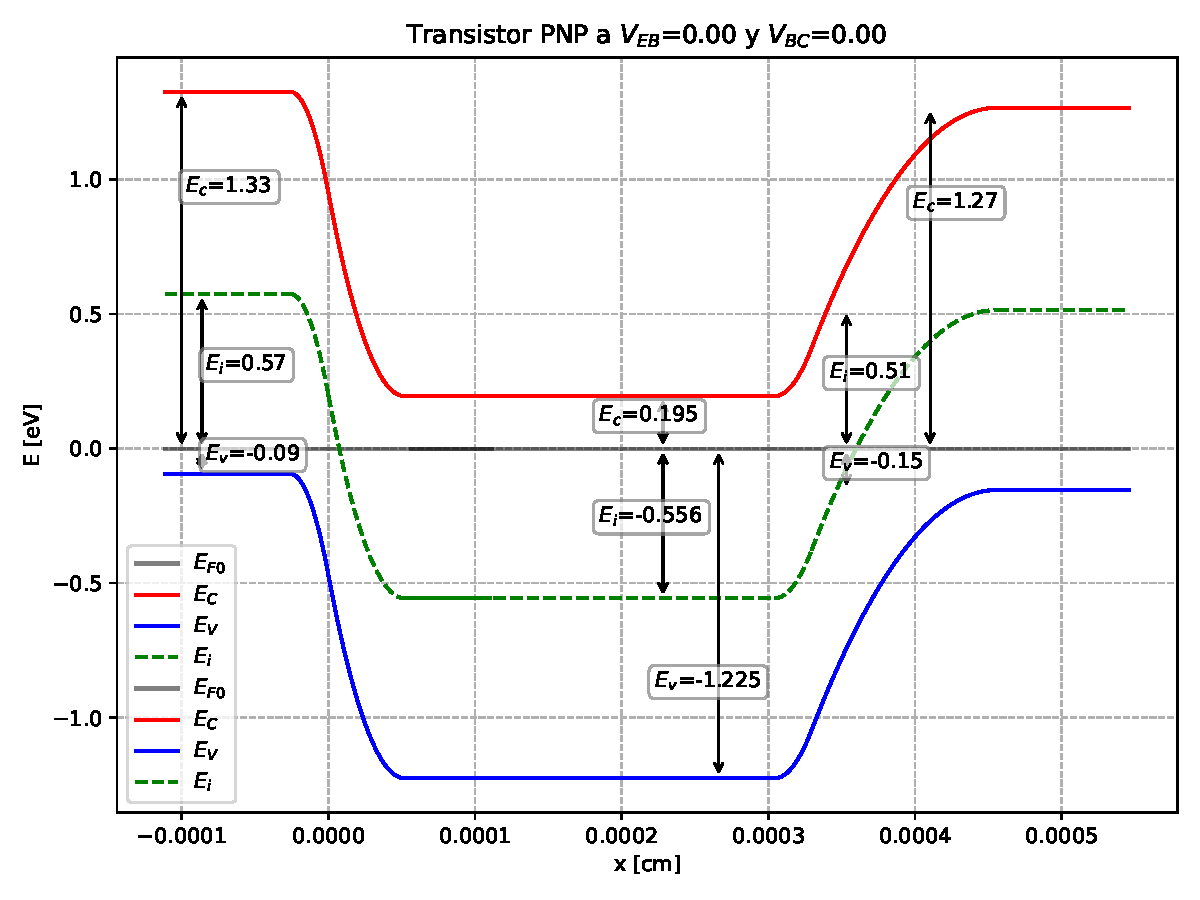
\includegraphics[width=0.48\linewidth]{Cuerpo/Ch_04/04_Ejercicio-2-01.pdf} \hfill
        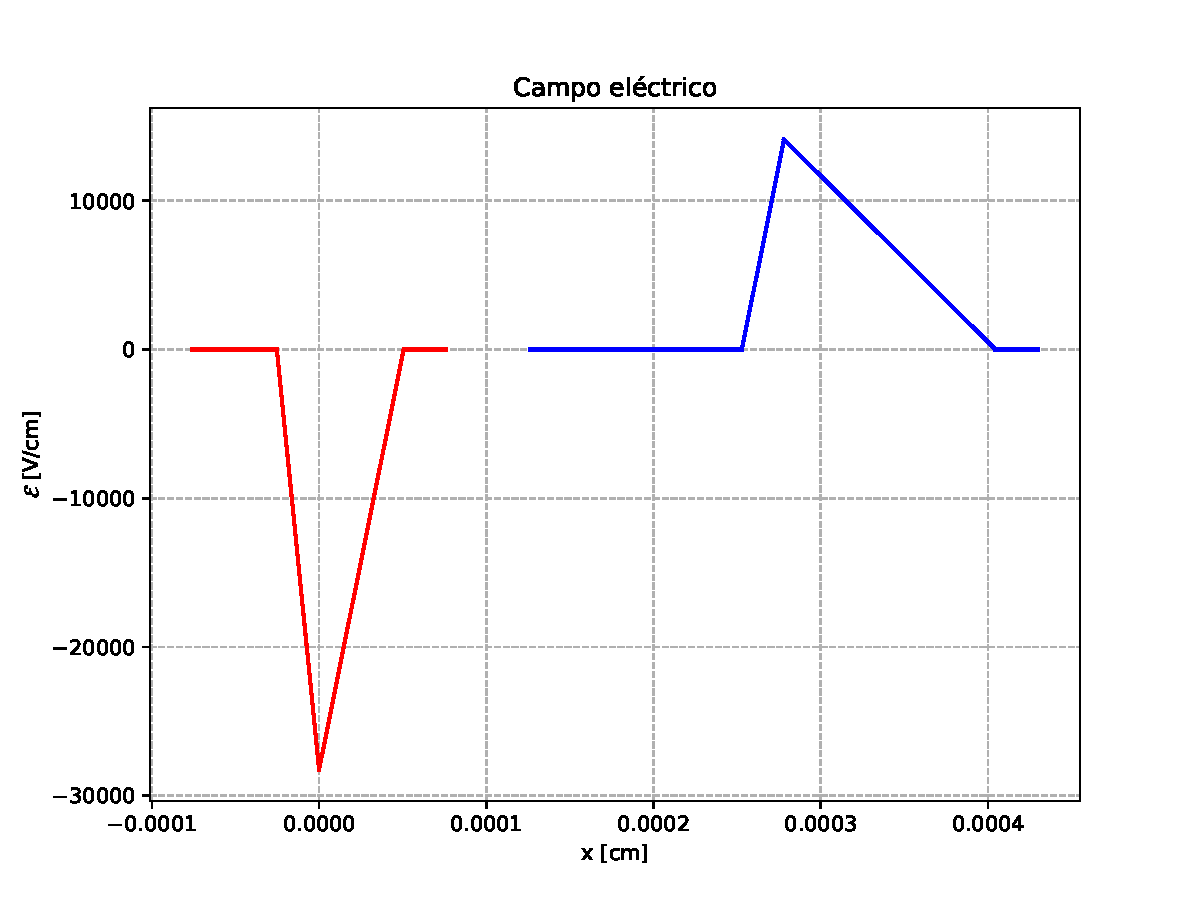
\includegraphics[width=0.48\linewidth]{Cuerpo/Ch_04/04_Ejercicio-2-03.pdf}
        \caption{Apartado a) imagenes.}
    \end{figure}
    \item Para la segunda tenemos que calcular los mismos paráemtros pero con polarizaciones
    \begin{equation}
        \text{EB:} \ x_n'=28.09 \ \mu \unit{m} \quad  x_p'=14.05  \mu \unit{m} \quad \Vbi'=1.13 \ \unit{V}
    \end{equation}
    \begin{equation}
        \text{BC:} \ x_n''=39.16 \ \mu \unit{m} \quad  x_p''=122.64  \mu \unit{m} \quad \Vbi'= 195.8 \ \unit{V}
    \end{equation}
    \noindent Y el campo eléctrico máximo
    \begin{equation}
       \abs{\Ecal'}_{\max}''=14200 \ \unit{V/cm} \quad  
       \abs{\Ecal''}_{\max}''=21900 \ \unit{V/cm} 
    \end{equation}
    \begin{figure}[h!] \centering
        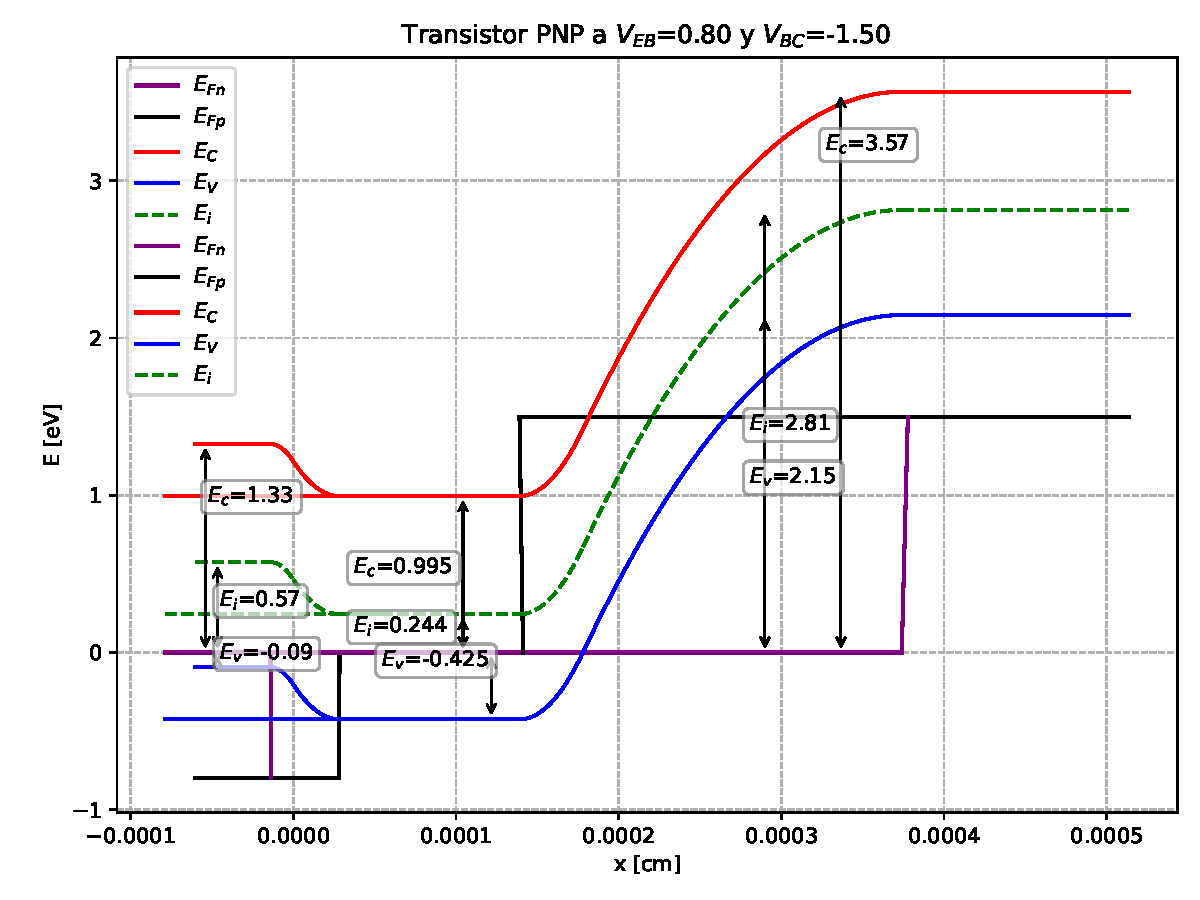
\includegraphics[width=0.48\linewidth]{Cuerpo/Ch_04/04_Ejercicio-2-02.pdf} \hfill
        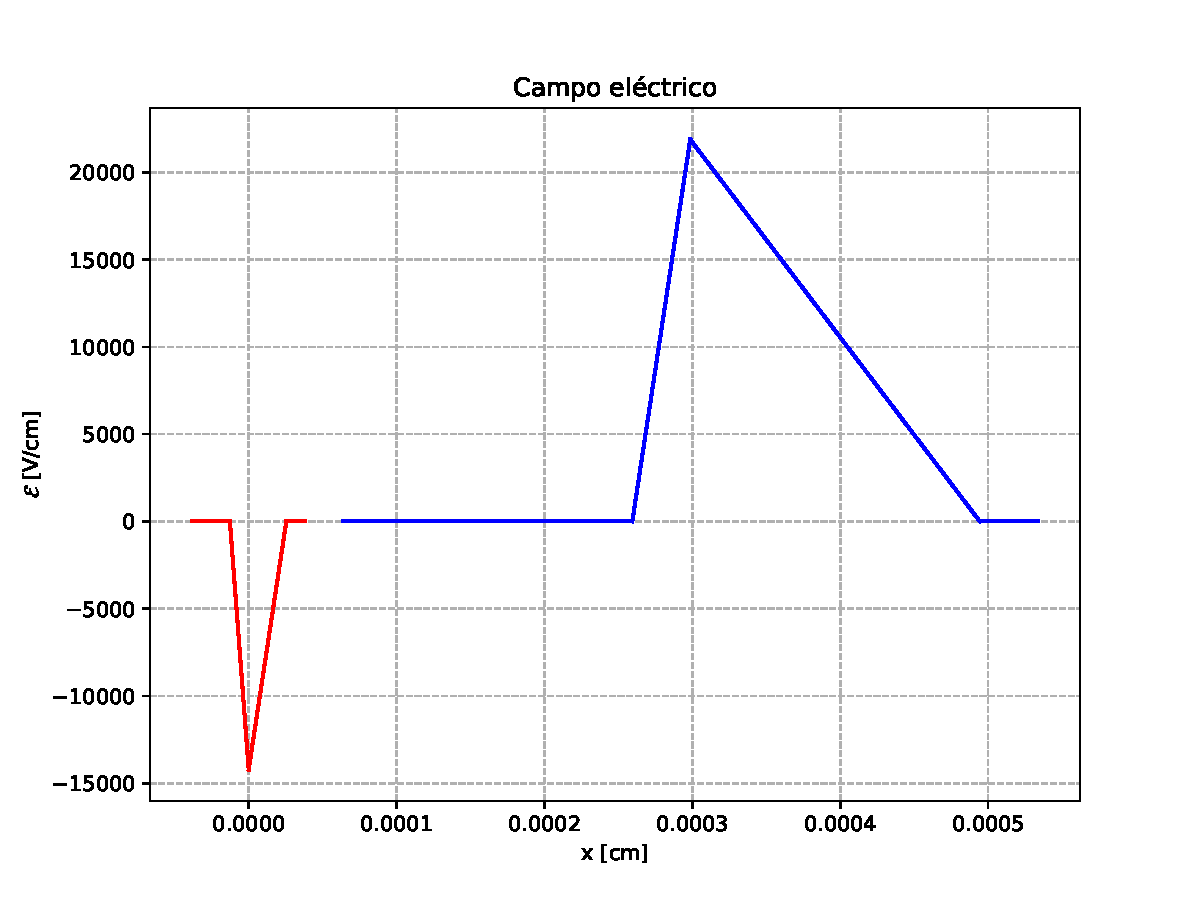
\includegraphics[width=0.48\linewidth]{Cuerpo/Ch_04/04_Ejercicio-2-04.pdf}
        \caption{Imagenes apartado b).}
    \end{figure}

\end{enumerate}
\vspace*{2em}

%---------------------------
% Ejercicio 3
%---------------------------

\begin{Enunciado}
\subsection*{Ejercicio 3} 
Tenemos un PNP de silicio con concentraciones $5 \times 10^{18}$, $3 \times 10^{17}$ y $1 \times 10^{16}$ cm\textsuperscript{-3}, con un ancho de emisor, base y colector de 20, 2 y 30 micras, y con un área de 1 cm\textsuperscript{2}. Cuando se polariza la unión emisor-base en directa con 0.5 voltios y la unión base-colector en inversa con 2 voltios, calcular y representar:
\begin{enumerate}[label=\alph*)]
    \item Las bandas bajo esa polarización.
    \item La concentración de minoritarios en el dispositivo.
    \item Calcular el valor de todas las componentes de corriente (suponiendo que no hay recombinación en la base), y representarlas gráficamente.
\end{enumerate}
\textbf{Datos:} concentración intrínseca $9.6 \times 10^9$ cm\textsuperscript{-3}, gap de energía 1.12 eV, masa del electrón 1.18 y de hueco 0.812, permitividad relativa: 11.8, permitividad del vacío: $8.85 \times 10^{-14}$ F/cm, coeficiente de difusión y tiempo de vida de emisor, base y colector de 52, 40 y 115 cm\textsuperscript{2}/s, y $10^{-8}$, $10^{-7}$ y $10^{-6}$ segundos.
\end{Enunciado}

\vspace*{1em}

\lipsum[1].

\vspace*{2em}

%---------------------------
% Ejercicio 4
%---------------------------

\begin{Enunciado}
\subsection*{Ejercicio 4} 
\lipsum[1].
\end{Enunciado}

\vspace*{1em}

\lipsum[1].

\vspace*{2em}
%---------------------------
% Ejercicio 5
%---------------------------

\begin{Enunciado}
\subsection*{Ejercicio 5}
\lipsum[1].
\end{Enunciado}

\vspace*{1em}
    
\lipsum[1]

\vspace*{2em}

%---------------------------
% Ejercicio 6
%---------------------------

\begin{Enunciado}
\subsection*{Ejercicio 6}
\lipsum[1].
\end{Enunciado}

\vspace*{1em}

\lipsum[1].
    
\vspace*{2em}
